Hashing, hash functions, hash tables, come into play when a compiler,
and in particular its parser, needs to store names (of identifiers)
and further information about the object of that name.

\Level 0 {Introduction}

A compiler, and in particular its parser, needs to store variables and
information about them. The data structure for this is in effect
addressed by the name of the variable, rather than by any numerical
index. This sort of storage is sometimes called `\index{associate
  storage}associative'. The design of a data structure for this is a
good example of trade-offs between efficiency and expediency.
\begin{itemize}
\item If variables are stored in the order in which they are
  encountered, storage is very fast, but searching will take time
  linear in the number of items stored.
\item If the list if kept sorted, searching for an item will take
  logarithmic time. However, insertion is now more expensive, taking linear
  time because all elements following have to be copied up.
\item A naively implemented linked list would give both insertion and
  retrieval time linearly in the number of stored items. In the
  insertion phase we avoid the copying, but finding the place to
  insert is harder, and in fact we can not use bisection here.
\item Items can be stored in a treewise fashion:
\begin{quote}
\Tree [.$\bullet$ [.B ART [.E GIN LL ] ] [.E LSE ND ] ]
\end{quote}
The cost of inserting and retrieving is then linear in the length of
the string, at least for as far as is necessary to disambiguate from
other strings.
\end{itemize}
These are then the issues we need to address:
\begin{itemize}
\item What is the cost of inserting a new item?
\item What is the cost of finding and retrieving an item?
\item What is the cost of deleting an item?
\end{itemize}

\Level 0 {Hash functions}

A hash function is function that maps non-numeric keys into a range of
integers, interpreted as the locations in a table. It would be nice if
this function was injective, to avoid mapping two keys to the same
location but  surprisingly hard, as is clear from the `birthday
paradox': it takes only 23 random picks from a 365-entry table to have
even chances of a collision. If we know all keys in advance, it is
possible to design a function that maps them uniquely into a table of
precisely the right size, but this is unrealistic, since the number of
possible keys in a programming language is very large, indeed unbounded.

\begin{figure}
\includegraphics[scale=.7]{hash-direct}
\caption{A hash function without conflicts}
\label{fig:hash-direct}
\end{figure}

A~`\index{Hash function}hash function' is then a function that maps
keys in some space to a range of integers~$0\ldots{M-1}$. A~good hash
function has the following properties:
\begin{itemize}
\item The hash value is fully determined by the data being hashed. For
  instance, it should not have a~`memory'.
\item The hash function uses as much as possible of the input
  data. Program variables often have names such as~\n{ikey}, so
  emphasis on the first letter is a bad idea.
\item The hash function "uniformly" distributes the data across the
  entire set of possible hash values.
\item The hash function generates very different hash values for
  similar strings. Variables like \n{key1}, \n{key2}, et cetera should
  not be mapped into a cluster.
\end{itemize}
Figure~\ref{fig:hash-direct} illustrates a hash function without conflicts.

Let us assume that we have found a way of mapping the names onto a
large integer space, for instance by interpreting the bit pattern of
the name as an integer. A~simple hash function would be
\begin{equation}
    h(K) = K\mod M, \label{eq:hash-div}\end{equation}
where $M$~is the size of the hash table.

Certain values of~$M$ are less desirable. For instance, if $M$~is
even, say~$M=2M'$, then the statement $r=K\mod M$ (say~$K=nM+r$ for
some~$n$) implies
\begin{eqnarray*}
K=2K'&\Rightarrow& r=2(nM'-K')\\
K=2K'+1&\Rightarrow& r=2(nM'-K')+1
\end{eqnarray*}
so the key is even, iff the original number is.
This places an undue influence on the last digit. If $M$~is a
multiple of~$3$, we find for numbers stored decimally or in bytes that
keys that are a permutation of each other get mapped to numbers that
differ by a multiple of~3, since both $10^n\mod 3=\nobreak1$ and
$2^8\mod 1=\nobreak1$.

\Level 1 {Multiplication and division strategies}

A good strategy is to take $M$~prime, and such that $r^k\not=\pm a\mod
M$, where $r$~the radix of the number system, and $a,k$~small.
(There is a list of suitable primes on
\url{http://planetmath.org/encyclopedia/GoodHashTablePrimes.html}.)

Equation~(\ref{eq:hash-div}) requires you to perform a division. The
same equation based on multiplication would use an integer~$A\approx\nobreak
w/M$, where $w$~is the maxint value. Then $1/M=A/w$, which is
simply~$A$ with an imaginary decimal point to its left. Observing that
\[ K\mod M=M(K/M\mod 1) \]
we define
\[ h(K)=\lfloor M\left(\left({A\over w}K\right)\mod
1\right)\rfloor. \]

As an example of the value of using a prime table size, consider
hashing the Bible, which consists of 42,829 unique words,
into an open hash table
with 30,241 elements (a prime number). In the end, 76.6 percent of the
slots were used and that the average chain was 1.85 words in length
(with a maximum of 6). The same file run into a hash table of 30,240
elements (evenly divisible by integers 2 through 9) fills only 60.7
percent of the slots and the average chain is 2.33 words long
(maximum: 10).

\Level 1 {String addition strategies}

One could Derive a hash key by adding or XORing together all bytes in
a string.
\begin{verbatim}
  h = <some value>
  for (i=0; i<len(var); i++)
    h = h + <byte i of string>;
\end{verbatim}
This runs into the problem that anagrams map into the same
key, and nearby strings into nearby keys. This could be remedied by
introducing a table of random numbers:
\begin{verbatim}
  h = <some value>
  for (i=0; i<len(var); i++)
    h = Rand( h XOR <byte i of string> );
\end{verbatim}
\begin{594exercise}
This algorithm only gives a one-byte key. How would you
derive longer keys? Give pseudo-code for the algorithm.
\end{594exercise}
\begin{answer}
Use this same method to derive two or more single-byte keys
\n{h1},~\n{h2}, et cetera, and combine these. You need to make sure that the
starting values for \n{h1},~\n{h2} are different.
\end{answer}

\Level 1 {Examples}

Here are a couple of published hash functions:
\begin{verbatim}
/* UNIX ELF hash
 * Published hash algorithm used in the UNIX ELF format for object files
 */
unsigned long hash(char *name)
{
    unsigned long h = 0, g;

    while ( *name ) {
        h = ( h << 4 ) + *name++;
        if ( g = h & 0xF0000000 )
          h ^= g >> 24;
        h &= ~g;
    }

}
\end{verbatim}
This hash key is then reduced to an index in the hash table by
\begin{verbatim}
#define HASHSIZE 997
    static int M = HASHSIZE;
    return h % M;
\end{verbatim}
Another hash function:
\begin{verbatim}
/* djb2
 * This algorithm was first reported by Dan Bernstein
 * many years ago in comp.lang.c
 */
unsigned long hash(unsigned char *str)
{
        unsigned long hash = 5381;
        int c; 
        while (c = *str++) hash = ((hash << 5) + hash) + c;
        return hash;
}
\end{verbatim}
Note the use of bit shifts to implement multiplication.

\Level 0 {Collisions}

The above techniques for generating randomly spread out addresses are
generally sufficient. The problem to worry about is how to handle
collisions, that is, if $h(k_1)=h(k_2)$ for different
keys~$k_1,k_2$. We will investigate several techniques for dealing
with this.

For all of the strategies below, any
performance analysis is statistical in nature. The average expected
behaviour is often excellent, but the worst case behaviour is always
very bad. In the worst case, all hash addresses map to the same
location, and search time is propertional to the number of elements in
the table.

The question is now how to find the storage locations for the elements
with conflicting hash keys. We will look at one strategy that
allocates space outside the hash table (`open hash table'), and two
that resolve the conflict by finding different locations in the table
(`closed hash table').

\Level 1 {Separate chaining}

A simple solution to hash conflicts is the create a linked list from
each table entry, as shown in figure~\ref{fig:hash-chain}.
\begin{figure}
\includegraphics[scale=.7]{hash-separate}
\caption{Separate chaining as a solution for hash conflicts}
\label{fig:hash-separate}
\end{figure}
This way of implementing a hash table is called `\index{separate
  chaining}separate chaining' or `\index{open hashing}open hashing'.
One problem with this approach is that we need to maintain two
different kinds of storage: static in the table and dynamic for the
linked lists.

The linked lists can be created by \n{malloc} (and released
by~\n{free}) calls. However, these are very expensive compared to
using a freespace pointer in a list. To amortize the cost, one could
allocate a block of cells, and dole them out gradually. The problem
with this strategy is dealing with deletions. If a cell is deleted,
rerouting the pointers is easy, but additionally we have to keep track
of which cells in the allocated chunk are free. This makes the open
hash table somewhat complicated to implement.

Another problem is that, while this strategy is fairly efficient if
the number of collisions is low, in order to get the number of
collisions low, one typically chooses the table size fairly large, and
then this solution is wasteful of storage. It is then better to store
all elements in the hash table and maintain links in the table.
\begin{594exercise}
Discuss the value of keeping the lists ordered by key: how does this
influence the run time of insertion and retrieval? Programming
languages like~C have local variables. Does this change your argument?
\end{594exercise}
\begin{answer}
In a list that is sorted, you do not have to search to the end. Your
average search time will be halved if the search is unsuccessful. If
the search is successful there will be no difference.

In languages with a block structure, data needs to be removed from the
list at the end of a block. It is then a better idea to organize data
by block level, with the innermost block at the front of the list. If
the blocklevel is included in the key (as most significant part), the
list will be organized this way by keeping it sorted.
\end{answer}

\Level 1 {Linear probing}

The easiest solution is to store a conflicting element in the location
immediately after the computed hash address.
\begin{figure}
\includegraphics[scale=.7]{hash-linear}
\caption{Linear probing as a solution for hash conflicts}
\label{fig:hash-linear}
\end{figure}
\begin{verbatim}
struct { ... } node;
node Table[M]; int Free;
/* insert K */
addr = Hash(K);
if (IsEmpty(addr)) Insert(K,addr);
else {
    /* see if already stored */
  test:
    if (Table[addr].key == K) return;
    else {
      addr = Table[addr].link; goto test;}
    /* find free cell */
    Free = addr;
    do { Free--; if (Free<0) Free=M-1; }
    while (!IsEmpty(Free) && Free!=addr)
    if (!IsEmpty(Free)) abort;
    else {
      Insert(K,Free); Table[addr].link = Free;}
}
\end{verbatim}

However, this is not the best solution. Suppose that the blocks of
size~$N$ is occupied, then the free pointer will search~$N/2$
locations on average for an address that maps into this block. While
this is acceptable, if two blocks coalesce, this makes the search time
double.  Note that the chance of the cell between two blocks filling
up is much larger than the chance of that exact address being
generated as hash: each hash in the top block will cause the address
to be filled.

\begin{figure}
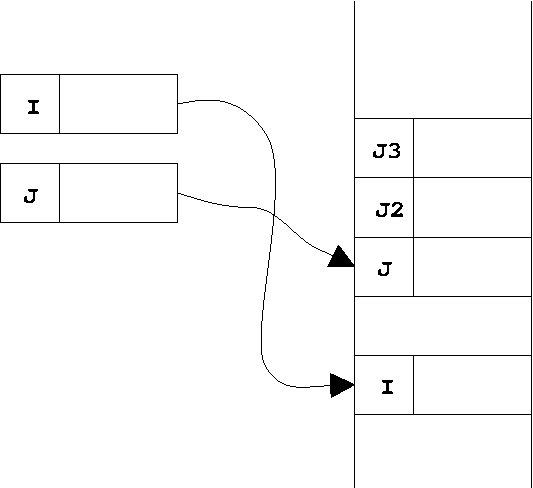
\includegraphics[scale=.3]{probing1}
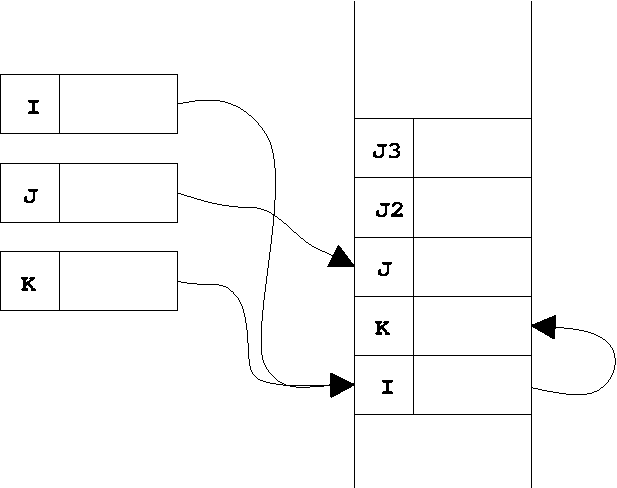
\includegraphics[scale=.3]{probing2}
\includegraphics[scale=.3]{probing3}
\caption{Coalescing of blocks in linear probing}
\label{fig:coalesce}
\end{figure}
This is illustrated in figure~\ref{fig:coalesce}. There is a gap of
size one between~$h(I)$ and a block starting at~$h(J)$. When a
conflict $h(K)=h(I)$ occurs, the free space pointer fills the
gap. A~subsequent conflict $h(L)=h(I)$ (or $h(L)=h(K)$) needs the free
space pointer to traverse the whole $J$~block to find the next
location.

With $\alpha=N/M$ the ratio between occupied cells and total table
size, the expected search time with this algorithm is
\[ T\approx\cases{
    {1\over 2}\left(1+\left({1\over 1-\alpha}\right)^2\right)&
        unsuccessful\cr
    {1\over 2}\left(1+{1\over 1-\alpha}\right)&
        successful\cr}
\]
It is clear that when $\alpha$~approaches~1, this time will go up
unbounded.

The clumping behaviour of this algorithm makes it sensitive to the
hash algorithm used. Care has to be taken that  successive keys, such
as \n{Ptr1},~\n{Ptr2}\dots, do not get mapped to successive hash
values~$K,K+1,\ldots$.

\Level 1 {Chaining}

The problems with linear probing can be prevented by storing
conflicting elements at the start or end of the table.
\begin{verbatim}
struct { ... } node;
node Table[M]; int Free = M;
/* insert K */
addr = Hash(K);
if (IsEmpty(addr)) Insert(K,addr);
else {
    /* see if already stored */
  test:
    if (Table[addr].key == K) return;
    else {
      addr = Table[addr].link; goto test;}
    /* find free cell */
    do { Free--; }
    while (!IsEmpty(Free)
    if (Free<0) abort;
    else {
      Insert(K,Free); Table[addr].link = Free;}
}
\end{verbatim}
This algorithm does the same list traversal as linear probing in the
case a search is ultimately successful. However, for an unsuccessful
search the \n{Free} pointer will usually be decreased by one, and only
occasionally by two or more, when it runs into already occupied
positions. Since these are likely to be spread out, having to search
more than two steps will be rare.
\begin{figure}
\includegraphics[scale=.3]{hash-chain0}
\includegraphics[scale=.3]{hash-chain}
\includegraphics[scale=.3]{hash-hash2}
\caption{Chaining as a solution for hash conflicts}
\label{fig:hash-chain}
\end{figure}

In this algorithm, occasionally a hash address will be an address that
has further links. We say that we have lists coalescing. This
increases search time slightly, but not by much, and preventing this
increases insertion time, because we would have to move cells.

With $\alpha=N/M$ the fraction of used to total table entries, find
that the number of entries searched is
\[ T\approx\cases{1+(e^{2\alpha}-1-2\alpha)/4&unsuccessful\cr
        1+(e^{2\alpha}-1-2\alpha)/8\alpha+\alpha/4&successful}
\]

The hash algorithm of \TeX\ is a variant of this chaining algorithm.

\Level 1 {Other solutions}

The solutions to the conflict problem given so far can be called
`\index{linear rehashing}linear rehashing'. The following strategies
are called `\index{nonlinear rehashing}nonlinear rehashing'. 
\begin{description}
\item[Random probing] Try $(h(m)+p_i)\mod s$, where $p_i$~is a
  sequence of random numbers. This requires either reproducible random
  numbers, or storing these numbers. In order to prevent colliding
  keys to collide on the next try too, the random number needs to
  depend on the key.
\item[Add the hash] Try $(i\times h(m))\mod s$. This requires~$s$ to be
  a prime number; with this approach clumping is prevented.
\end{description}
They have
the advantage that occupied locations in the table remain fairly scattered.
On the other hand, they require further hash calculations. Also,
because of the irregular memory access pattern, the cost of memory
operations may become significant here.

\Level 1 {Deletion}

A surprising aspect of closed hash table algorithms is that generally it is
hard to delete elements. Since most algorithms give coalescing lists,
we can not mark a cell empty if its key is to be removed. Instead, we
mark a cell `deleted', which removes the key, but leaves the link intact.
There are algorithms that can deal with deletions, but they have a
fairly high complexity.

On the other hand, deleting in an open hash table algorithm is
simple. The complication there is the freeing of the memory. If the
cells are allocated in chunks, the decision to free a chunk becomes
complicated.

\Level 0 {Other applications of hashing}

The foremost application of hashing is in compilers. However, there
are other uses.

\Level 1 {Truncating searches}

In applications such as chess programs, you want to avoid evaluating a
configuration twice if it's arrived at two different ways. This can be
done by storing evaluations in a table. This table can be addressed by
the configuration as a key itself, but these keys are long and span a
large space, so searching will probably be expensive. Instead, one can
use a hash table.

If two
configurations generate the same hash key, they can be, but need not
be the same, so further decision might be needed. To avoid this second
stage work, a~good quality hash function is essential.

(This example comes from
\url{http://www.seanet.com/~brucemo/topics/hashing.htm}.)

\Level 1 {String searching}

The question `does a string of length~$M$ appear anywhere in a
document of length~$N$' can be answered in $O(NM)$ time by a sequence
of string comparisons. However, we can do considerably better,
reducing the complexity to~$O(N+M)$.

A hash function that adds characters together will give the same hash
key for strings that are anagrams of each other. This means that
instead of doing a string comparison we can compare hash keys, and
only if they are equal resort to a full string comparison. To get the
complexity down, we note that if the hash function is of the form
\[ h(k)=\left\{\sum_ik[i]\right\}\mathop{\mathrm{mod}} K,\]
where $k$ is a character string,
then (for a text~$t$ long enough)
\[ h(t[2\ldots n+1]) = h(t[1\ldots n])+t[n+1]-t[1] \]
(with addition/subtraction modulo~$K$)
so we can cheaply update the hash key in $O(1)$ time.

\Level 0 {Discussion}

In a comparison between hash tables and, for instance, tree-based
storage, there is no clear preference. Hash tables can be faster,
because, until the table fills up, access is~$O(1)$. A~similar
complexity can be obtained for trees, but
\begin{itemize}
\item memory access in trees is more chaotic, leading to worse cache
  or paging behaviour;
\item memory is allocated and freed dynamically; circumventing that
  takes considerable programming effort;
\item trees can become unbalanced, and balancing them is tricky to
  program, and takes time;
\item the optimal search time can be made approximately equal, but
  that is again hard to code.
\end{itemize}

Closed hash tables have the advantage of simpler storage management,
and, until they fill up, no worse performance than open tables.
